\documentclass[11pt]{article}
\usepackage[usenames, dvipsnames]{color}
\usepackage[margin=1in,vmargin=1in]{geometry}
\usepackage[utf8]{inputenc}
\usepackage[english]{babel}
\usepackage{tikz}
\usepackage{pgfplots}
\usepackage{fancyhdr}
\usepackage{comment}
\pagestyle{fancy}
\usepackage{url}
\usepackage[font=small,labelfont=bf,labelsep=period]{caption}
\usepgfplotslibrary{polar}
\usepgflibrary{shapes.geometric}
\usetikzlibrary{calc}
\pgfplotsset{compat=1.5.1}
\pgfmathdeclarefunction{gauss}{2}{%
  \pgfmathparse{1/(#2*sqrt(2*pi))*exp(-((x-#1)^2)/(2*#2^2))}%
}

\pgfmathdeclarefunction{bivar}{4}{%
  \pfgmathparse{1/(2*pi*#2*#4) * exp(-((x-#1)^2/#2^2 +
    (y-#3)^2/#4^2))/2}%
}
\usetikzlibrary{shadows}
\usepackage{graphicx}
\usepackage{graphics}
\usepackage[mode=buildnew]{standalone}
\usepackage{amsmath}
\usepackage{amsthm}
\usepackage{amssymb}
\usepackage{float}
\usepackage{hyperref}
\DeclareMathOperator*{\argmin}{arg\,min}
\newcommand*{\everymodeprime}{\ensuremath{\prime}}
\graphicspath{{figs/}}

\title{Label Smoothing with Graph Convolution}
\author{}
\date{}

\begin{document}

\maketitle

\section{Graph Convolution}

Most algorithms seem to be doing variants of the same general algorithm. I think it is a good exercise for me to go through some of these papers and explain how they related to each other in the context of probabilistic modeling. The goal is to clearly outline the relationships among these different algorithms to more clearly see a way to contribute to this area.

% table comparing methods in papers. for example, organize the more recent publications on the clothing1m dataset into a table
% identify the top noisy label/label smoothing papers
% graphconv + knn + update (main idea); run a simple algorithm on mnist
% 

\vspace{2cm}
\noindent Some take-aways from reading papers thus far
\begin{itemize}
\item It seems that utilizing information during the learning process is a new research area with some room to publish. That seems promising for us using GraphConvolution to regularize the deep learning model
\item I'm not convinced noisy labels is a direct problem that needs direct fixing; e.g. recovering a "groundtruth" may not be important for getting good estimates of deep learning parameters. MNIST and Cifar does remarkably well even with high label noise.
\item this area seems busy! there must be something we can do in this area.
\item I think using GraphConv to regularize the loss function would be analogous to some type of ``perceptual loss'' function people use currently. I think we would have to compare to ``regularized classification'' methods as well, rather than just ``noisy labels'' papers. I think it is \emph{very popular} to use the final representations of a neural network to inform some part of learning or testing. I think we need to widen the related literature scope to understand if we are calling ``noisy labels'' by the wronge name; e.g. simply training to find good representations implies we perform the same algorihm as our proposed one. This means we would taking PAPER X's algorithm (ALG X) and applying it to ``noisy labels'' (APPLICATION Y) and our contribution would be limited to (i) identifying ALG X can be applied to APPLICATION Y and (ii) maybe providing some justifiction for such appilcations. Is this enough of a paper? This seems weak to me.
\end{itemize}

\vspace{2cm}
\noindent Other tasks I am looking to complete are:
\begin{itemize}
\item Code up some Graph convolution (complete)
\item Understand how collaborative filtering relates to markov random fields
\end{itemize}

\begin{figure}[h]
  \centering
  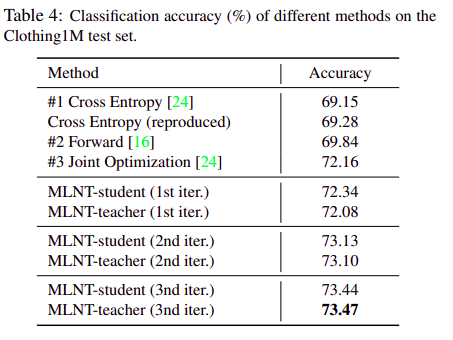
\includegraphics[width=0.5\linewidth]{cvpr2019_learning_to_learn_w_noisy_data}
  \caption{Clothing 1M Result from cvpr2019 ``learning to learn with noisy data''. Ref 24 is cvpr2018 ``Joint optimization framework for learning with noisy labels.'' Ref 16 is cvpr 2017 ``Making deep neural networks robust to label noise: A loss correction approach.''}
\end{figure}

\begin{figure}[h]
  \centering
  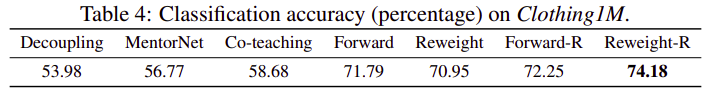
\includegraphics[width=0.8\linewidth]{neurips2019_anchor_points}
  \caption{Clothing 1M Result from neurips2019 ``Are Anchor Points Really Indispensable in Label-Noise Learning?''. neurips 2018 ``Decoupling'' = ``Decoupling "when to update" from "how to update"... }
\end{figure}


\clearpage
\newpage
\section{References}



\noindent {\bf *Learning Graph Neural Networks with Noisy Labels }

\noindent ICLR 2019

\noindent Citations: 1

\noindent Relevance Score: 10

\noindent Comparison Needed?: yes.

\noindent Tags: transition matrix estimation, graph convolution

\begin{itemize}
\item this is graph convolution for label denoising.
\end{itemize}

\vspace{2cm}
\noindent {\bf *Graph Convolutional Label Noise Cleaner:
Train a Plug-and-play Action Classifier for Anomaly Detection }

\noindent CVPR 2019

\noindent Citations: 3

\noindent Relevance Score: 10

\noindent Comparison Needed?: maybe.

\noindent Tags: transition matrix estimation, graph convolution

\begin{itemize}
\item this is graph convolution for label denoising.
\end{itemize}


\vspace{2cm}
\noindent {\bf *Are Anchor Points Really Indispensable in Label-Noise Learning?}

\noindent NeurIPs 2019

\noindent Citations: 6

\noindent Relevance Score: 10

\noindent Comparison Needed?: yes.

\noindent Tags: transition matrix estimation

\noindent Url: \url{https://arxiv.org/pdf/1906.00189.pdf}

\begin{itemize}
\item reading this is nice, great writing. clear experiments and algorithms.
\item Risk and Classification statistically consistent methods rely on transition matrices. 
\item Existing theories have shown that the transition matrix can be learned by exploiting anchor points
\item when there are no anchor points, the transition matrix will be poorly learned
\item without employing anchor points, we propose a transition-revision (T-Revision) method to effectively learn transition matrices
\item we first initialize it by exploiting data points that are similar to anchor points, having high noisy class posterior probabilities. Then, we modify the initialized matrix by adding a slack variable, which can be learned and validated together with the classifier by using noisy data
\end{itemize}

\vspace{2cm}\noindent {\bf Combinatorial Inference against Label Noise}

\noindent NeurIPs 2019

\noindent Citations: 0

\noindent Relevance Score:

\noindent Comparison Needed?: 

\noindent Tags:

\begin{itemize}
  \item a unique classification framework of constructing multiple models in heterogeneous coarse-grained meta-class spaces and making joint inference of the trained models for the final predictions in the original (base) class space.
  \item improvement via constructing meta-classes and improves accuracy via combinatorial inferences over multiple constituent classifiers
  \item distinct and complementary properties for the given problem, we can even incorporate additional off-the-shelf learning algorithms to improve accuracy further
  \item techniques to organize multiple heterogeneous meta-class sets using k-means clustering and identify a desirable subset leading to learn compact models
  \item curriculum learning seems to include either (i) re-ordering sampls or (ii) re-weighting samples.
\end{itemize}

\vspace{2cm}\noindent {\bf L\_DMI: A Novel Information-theoretic Loss Function for Training Deep Nets Robust to Label Noise}

\noindent NeurIPs 2019

\noindent Citations: 6

\noindent Relevance Score: 5

\noindent Comparison Needed?: No

\noindent Tags: information theoretic analysis for label noise

\begin{itemize}
  \item most methods only handle limited kinds of noise patterns, require auxiliary information or steps (e.g., knowing or estimating the noise transition matrix), or lack theoretical justification. 
  \item novel information-theoretic loss function, LDMI, for training deep neural networks robust to label noise
  \item generalized version of mutual information, termed Determinant based Mutual Information (DMI), which is not only information-monotone but also relatively invariant.
  \item provably robust to instance-independent label noise, regardless of noise pattern, and it can be applied to any existing classification neural networks straightforwardly without any auxiliary information
\end{itemize}


\vspace{2cm}\noindent {\bf Robust Inference via Generative Classifiers for Handling Noisy Labels}

\noindent ICML 2019

\noindent Citations: 7

\noindent Relevance Score:

\noindent Comparison Needed?: 

\noindent Tags:

\noindent Url: \url{https://arxiv.org/pdf/1901.11300.pdf}

\begin{itemize}
  \item induce a generative classifier on top of hidden feature spaces of the pre-trained DNNs, for obtaining a more robust decision boundary
  \item By estimating the parameters of generative classifier using the minimum covariance determinant estimator, we significantly improve the classification accuracy with neither re-training of the deep model nor changing its architectures
  \item assumption of Gaussian distribution for features, we prove that RoG generalizes better than baselines under noisy labels.
  \item we propose the ensemble version of RoG
\end{itemize}


\vspace{2cm}\noindent {\bf Unsupervised Label Noise Modeling and Loss Correction}

\noindent ICML 2019

\noindent Citations: 13

\noindent Relevance Score:

\noindent Comparison Needed?: 

\noindent Tags:

\noindent Url: \url{https://arxiv.org/pdf/1904.11238.pdf}

\begin{itemize}
  \item two-component mixture model as an unsupervised generative model of sample loss values during training to allow online estimation of the probability that a sample is mislabelled. 
  \item beta mixture to estimate this probability and correct the loss by relying on the network prediction (the so-called bootstrapping loss).
  \item We further adapt mixup augmentation to drive our approach a step further; mixing two classes in raw pixel space
\end{itemize}

\vspace{2cm}\noindent {\bf How does Disagreement Help Generalization against Label Corruption?}

\noindent ICML 2019

\noindent Citations: 18

\noindent Relevance Score: 8

\noindent Comparison Needed?: Maybe

\noindent Tags: Co-teaching

\begin{itemize}
\item 
\end{itemize}

\vspace{2cm}\noindent {\bf Learning to Learn from Noisy Labeled Data}

\noindent CVPR 2019

\noindent Citations: 26

\noindent Relevance Score:

\noindent Comparison Needed?: 

\noindent Tags: learning dynamics

\noindent Url: \href{https://arxiv.org/pdf/1812.05214.pdf}{url}

\begin{itemize}
  \item meta-learning update is performed prior to conventional gradient update.
  \item proposed meta-learning method simulates actual training by generating synthetic noisy labels, and train the model such that after one gradient update using each set of synthetic noisy labels
\end{itemize}



\vspace{2cm}\noindent {\bf Deep k-Nearest Neighbors: Towards Confident,
Interpretable and Robust Deep Learning}

\noindent CoRR 2018

\noindent Citations: 96

\noindent Relevance Score:

\noindent Comparison Needed?: 

\noindent Tags: 

\begin{itemize}
  \item 
\end{itemize}

\vspace{2cm}\noindent {\bf To Trust Or Not To Trust A Classifier}

\noindent NeurIPs 2018

\noindent Citations: 54

\noindent Relevance Score:

\noindent Comparison Needed?: 

\noindent Tags: 

\begin{itemize}
  \item 
\end{itemize}

\vspace{2cm}\noindent {\bf Co-teaching: Robust Training of Deep Neural Networks with Extremely Noisy Labels}

\noindent NeurIPs 2018

\noindent Citations: 130

\noindent Relevance Score:

\noindent Comparison Needed?: 

\noindent Tags:

\noindent Url: \href{https://arxiv.org/pdf/1804.06872.pdf}{url}

\begin{itemize}
\item first memorize training data of clean labels and then those of noisy labels
\item a new deep learning paradigm called “Co-teaching” for combating with noisy labels
\item we train two deep neural networks simultaneously, and let them teach each other given every mini-batch:
\item firstly, each network feeds forward all data and selects some data of possibly clean labels
\item  secondly, two networks communicate with each other what data in this mini-batch should be used for training;
\item finally, each network back propagates the data selected by its peer network and updates itself
\end{itemize}

\vspace{2cm}\noindent {\bf Robustness of conditional GANs to noisy labels}

\noindent NeurIPs 2018

\noindent Citations: 17

\noindent Relevance Score:

\noindent Comparison Needed?: 

\noindent Tags:

\noindent Url: \href{https://papers.nips.cc/paper/8229-robustness-of-conditional-gans-to-noisy-labels.pdf}{url}

\begin{itemize}
  \item learning conditional generators from noisy labeled samples, where the labels are corrupted by random noise
  \item standard training of conditional GANs will not only produce samples with wrong labels, but also generate poor quality samples
  \item We consider two scenarios, depending on whether the noise model is known or not.
  \item known noise: introduce a novel architecture RCGAN. The main idea is to corrupt the label of the generated sample before feeding to the adversarial discriminator, forcing the generator to prouce samples with clean labels
  \item unknown noise: we provide an extension of our architecture, which we call RCGAN-U
\end{itemize}

\vspace{2cm}\noindent {\bf Masking: A New Perspective of Noisy Supervision}

\noindent NeurIPs 2018

\noindent Citations: 30

\noindent Relevance Score: 10

\noindent Comparison Needed?: Yes

\noindent Tags: block diagonal graph, gan, 

\begin{itemize}
\item in summary, the idea seems reasonable and I actually kind of like it. I think the rationalization for their method is very strange. The add an auxiliary variable into the transition matrix model called a "structure" variable. The experiments seem insufficient. very preachy ugh
\item readable writing. i don't like their reasoning though
\item great literature review.
\item they don't seem to justify themselves against competing method very well
\item the idea is to use the fact that people will forget to tag regions. If they are tagging a mountain range and beach, those will not be confused. But they may forget to tag the "dog" on the "beach" scene.
\item Their use of reference 9 is questionable; I don't know if 9 implies their claim of "both approaches introduce a permanent regularization
bias, and the learned classier barely reaches the optimal performance"
\item corruption of labels via unknown noise transition matrix.
\item by estimating this matrix, classifiers can escape from overfitting those noisy labels. such estimation is practically difficult
\item human-assisted approach called “Masking” that conveys human cognition of invalid class transitions and naturally speculates the structure of the noise transition matrix
\item structure-aware probabilistic model incorporating a structure prior, and solve the challenges from structure extraction and structure alignment
\item only estimate unmasked noise transition probabilities and the burden of estimation is tremendously reduced
\item weird justification for why jointly learning noise and params is bad: "brute-force learning leads to inexact estimation due to a finite dataset."
\end{itemize}

\vspace{2cm}\noindent {\bf Co-Teaching: Robust training of deep neural networks with extremely noisy labels.}

\noindent NeurIPs 2018

\noindent Citations: 130

\noindent Relevance Score:

\noindent Tags:

\begin{itemize}
\item focuses on training on
selected samples
\item they personify optimization algorithms, minus points from me: "... they can ask peer classmates to
review their papers..."
\item the writing of this paper is a bit weird
\item exchange the selected small-loss instances,
i.e., update parameters in f (resp. g) using mini-batch instances selected from g 
\item different
abilities to filter out the label noise
\item how is this different from "bagging"
\end{itemize}

\vspace{2cm}\noindent {\bf Using Trusted Data to Train Deep Networks on Labels Corrupted by Severe Noise}

\noindent NeurIPs 2018

\noindent Citations: 77

\noindent Relevance Score:

\noindent Comparison Needed?: 

\noindent Tags:

\begin{itemize}
\item previous works assume that no source of labels can be trusted. 
\item we relax this assumption and assume that a small subset of the training data is trusted
\item substantial label corruption robustness performance gains.
\item particularly severe label noise can be combated by using a set of trusted data with clean labels.
\end{itemize}

\noindent comments:
\begin{itemize}
\item this seems closest to the mrf model
\end{itemize}

\vspace{2cm}\noindent {\bf Generalized Cross Entropy Loss for Training Deep Neural Networks with Noisy Labels}

\noindent NeurIPs 2018

\noindent Citations: 150

\noindent Relevance Score:

\noindent Comparison Needed?: 

\noindent Tags:

\noindent Url: \href{https://papers.nips.cc/paper/8094-generalized-cross-entropy-loss-for-training-deep-neural-networks-with-noisy-labels.pdf}{url}

\begin{itemize}
\item mean absolute error (MAE) has recently been proposed as a noise-robust alternative to the commonly-used categorical cross entropy (CCE) loss.
\item shown here, MAE can perform poorly with DNNs and challenging datasets
\item we present a theoretically grounded set of noise-robust loss functions that can be seen as a generalization of MAE and CCE.
\end{itemize}

\vspace{2cm}\noindent {\bf Robot Learning in Homes: Improving Generalization and Reducing Dataset Bias}

\noindent NeurIPs 2018

\noindent Citations: 25

\noindent Relevance Score: 3

\noindent Comparison Needed?: No

\noindent Tags: application of noisy labels

\begin{itemize}
\item data collected using low cost robots suffer from noisy labels due to imperfect execution and calibration errors.
\item To handle this, we develop a framework which factors out the noise as a latent variable
\item Use direct optimization to learn join of $p(\hat{y},y|x)$ from Misera 2015.
\end{itemize}

\vspace{2cm}\noindent{\bf Masking: A new perspective of noisy supervision.}

\noindent NeurIPs 2018

\noindent Citations: 30

\noindent Relevance Score:

\noindent Comparison Needed?: 

\noindent Tags: noise transition matrix, restricting feasible set

\begin{itemize}
\item nice writing its easy to read
\item taught me about "sample selection bias"
\item makes the problem tractable by removing elements from the search space
\item Masking restricts the set of feasible transition matrices using a structure-aware probabilistic model
\item structure prior for solving structure extraction
and structure alignment
\item only estimate unmasked noise
transition probabilities 
\item 
\end{itemize}

\vspace{2cm}\noindent {\bf Learning to Reweight Examples for Robust Deep Learning}

\noindent ICML 2018

\noindent Citations: 162

\noindent Relevance Score:

\noindent Comparison Needed?: 

\noindent Tags:

\noindent Url: \href{https://arxiv.org/pdf/1803.09050.pdf}{url}

\begin{itemize}
  \item learns to assign weights to training examples based on their gradient directions.
  \item meta gradient descent step on the current mini-batch example weights (which are initialized from zero) to minimize the loss on a clean unbiased validation set.
  \item an any type of deep network, does not require any additional hyperparameter tuning
  \item on class imbalance and corrupted label problems where only a small amount 
\end{itemize}

\begin{itemize}
\item They use the same latent space representation of the real label as I do
\end{itemize}

\vspace{2cm}\noindent {\bf MentorNet: Learning Data-Driven Curriculum for Very Deep Neural Networks on Corrupted Labels}

\noindent ICML 2018

\noindent Citations: 189

\noindent Relevance Score: 10

\noindent Comparison Needed?: Yes

\noindent Tags: curriculum learning, weighting samples

\begin{itemize}
\item create MentorNet to supervise training of StudentNet
\item MentorNet provides a curriculum (sample weighting scheme) for StudentNet to focus on the sample
the label of which is probably correct
\item MentorNet learns a data-driven
curriculum dynamically with StudentNet
\item existing
curriculums are usually predefined and remain fixed during
training, ignoring the feedback from the student.
\item I have a hard time believing the above statement 
\item Second, the alternating minimization, commonly used in
CL and self-paced learning (Kumar et al., 2010) requires
alternative variable updates, which is difficult for training
very deep CNNs via mini-batch stochastic gradient descent.
\item I don't understand the above issue at all; isn't this very simply?
\item the learning objective is jointly minimized
using MentorNet and StudentNet via mini-batch stochastic
gradient descent.
\item There should be some better language for discussion curriculum learning in terms of probabilistic distributions. This may help us find more work.
\end{itemize}


\vspace{2cm}\noindent {\bf Dimensionality-Driven Learning with Noisy Labels}

\noindent ICML 2018

\noindent Citations: 75

\noindent Relevance Score:

\noindent Comparison Needed?: 

\noindent Tags: learning dynamics

\begin{itemize}
\item a new perspective for understanding DNN generalization for such datasets, by investigating the dimensionality of the deep representation subspace of training samples
\item from a dimensionality perspective, DNNs exhibit quite distinctive learning styles when trained with clean labels versus when trained with a proportion of noisy labels
\item a new dimensionality-driven learning strategy, which monitors the dimensionality of subspaces during training and adapts the loss function accordingly
\item uses k-nn
\end{itemize}

\vspace{2cm}\noindent {\bf Learning with biased complementary labels}

\noindent ICCV/ECCV 2018

\noindent Citations: 47

\noindent Relevance Score:

\noindent Comparison Needed?: 

\noindent Tags:

\begin{itemize}
\item 
\end{itemize}

\vspace{2cm}\noindent {\bf Curriculumnet: Weakly supervised learning from large-scale web images.}

\noindent ICCV/ECCV 2018

\noindent Citations: 47

\noindent Relevance Score: 8

\noindent Comparison Needed?: No

\noindent Tags: build a dataset, density estimation of data, curriculum, clustering, k-means

\begin{itemize}
\item I feel this paper is missing several experiments.
\item MentorNet is the "deep learning" version of this
\item raining deep neural networks on large-scale weakly-supervised web images,
which are crawled raw from the Internet by using text queries, without any human annotation.
\item principled learning strategy
by leveraging curriculum learning
\item targets noisy labels and data imbalance
\item  measuring the complexity of data using
its distribution density in a feature space, and rank the complexity in
an unsupervised manner
\item  density based
clustering algorithm that measures the complexity of training samples
\item implicit graph structure created to run k-means
\item the order of the curriculum learning is done by sorting the probabilities associated with each cluster; e.g. the "tighter" cluster is consider "easy" and a distributed cluster is considered "hard"
\item I also feel like papers like this should compare with dataset augmentation to account for inflated results when adding more data. Dataset augmentation only works in a limited region, so it is for sure computable; I see little reason why they don't inclue this
\item Additionally, the do not run ablation study randomizing either (i) the clusters or (ii) the order of the curriculum. It is unclear to me how the order of the cluster, size of the cluster, or metrics of cluster "goodness" play a role into the quality of curriculum learning.
\end{itemize}


\vspace{2cm}\noindent {\bf Exploring the Limits of Weakly Supervised Pretraining}

\noindent ICCV/ECCV 2018

\noindent Citations: 229

\noindent Relevance Score:

\noindent Comparison Needed?: 

\noindent Tags:

\begin{itemize}
\item DNN trained to predict hashtags on billions of social media images.
\item not really noisy labels
\end{itemize}

\vspace{2cm}\noindent {\bf CurriculumNet: Weakly Supervised Learning from Large-Scale Web Images}

\noindent ICCV/ECCV 2018

\noindent Citations: 47

\noindent Relevance Score: 7

\noindent Comparison Needed?: No

\noindent Tags:

\begin{itemize}
\item We develop a principled learning strategy by leveraging curriculum learning, with the goal of handling a massive amount of noisy labels and data imbalance effectively.
\item measuring the complexity of data using its distribution density in a feature space, and rank the complexity in an unsupervised manner.
\item where the negative impact of noisy labels is reduced substantially
\item highly noisy labels can improve testing accuracy by serving as regularization
\end{itemize}

\vspace{2cm}\noindent {\bf Deep Learning is Robust to Massive Label Noise (rejected from iclr 2018; referenced in iclr 2019 reject as "worth reading")}

\noindent ICLR 2018

\noindent Citations: 145

\noindent Relevance Score: 7

\noindent Comparison Needed?: 

\noindent Tags:

\begin{itemize}
\item show deep neural networks are capable of generalizing from training data for which true labels are massively outnumbered by incorrect labels.
\item demonstrate remarkably high test performance after training on corrupted data from MNIST, CIFAR, and ImageNet.
\item For example, on MNIST we obtain test accuracy above 90 percent even after each clean training example has been diluted with 100 randomly labeled examples.
\item We show that training in this regime requires a significant but manageable increase in dataset size that is related to the factor by which correct labels have been diluted.
\item a result shows how increasing noise decreases the effective batch size.
\item in fact, to my point about not needing explicity label denoising, we have "Revisiting Unreasonable Effectiveness of Data in Deep Learning Era" demonstrating a logarithmic growth of dataset size
\end{itemize}

\vspace{2cm}\noindent {\bf Learning From Noisy Singly-labeled Data}

\noindent ICLR 2018

\noindent Citations: 43

\noindent Relevance Score: 4

\noindent Comparison Needed?: 

\noindent Tags:

\begin{itemize}
\item not closely relevant to our project goals.
\item how to optimally learn from multiple noisy workers?
\item how to allocate labeling budget to maximum classifier performance?
\item propose a new algorithm for jointly modeling labels and worker quality from noisy crowd-sourced data
\item alternating minimization proceeds in rounds, estimating worker quality from disagreement with the current model and then updating the model by optimizing a loss function that accounts for the current estimate of worker quality. (EM algorithm)
\item even with only one annotation per example, our algorithm can estimate worker quality.
\end{itemize}

\vspace{2cm}\noindent {\bf FIDELITY-WEIGHTED LEARNING}

\noindent ICLR 2018

\noindent Citations: 

\noindent Relevance Score: 

\noindent Comparison Needed?: 

\noindent Tags: sample re-weighting

\begin{itemize}
\item
\end{itemize}


\vspace{2cm}\noindent {\bf Robust active label correction}

\noindent AISTAT 2018

\noindent Citations: 5

\noindent Relevance Score: 6

\noindent Comparison Needed?: 

\noindent Tags:

\begin{itemize}
\item this uses expected model change for the new label
\item e.g. this uses gradient information or learning dynamics
\item this paper is confusing to me. I am not a big fan of the writing
\item 
\end{itemize}




\vspace{2cm}\noindent {\bf Smooth Neighbors on Teacher Graphs for Semi-supervised Learning}


\noindent CVPR 2018 (spotlight)

\noindent Citations: 70

\noindent Relevance Score: 

\noindent Comparison Needed?: 

\noindent Tags: manifold learning, 

\begin{itemize}
\item contrasts self-ensembling
\item 
\end{itemize}

\vspace{2cm}\noindent {\bf Joint Optimization Framework for Learning With Noisy Labels}

\noindent CVPR 2018

\noindent Citations: 100

\noindent Relevance Score: 10

\noindent Comparison Needed?: Yes

\noindent Tags:

\begin{itemize}
\item pretty okay idea
\item the writing is silly: "To address this problem, commonly used regularization techniques including dropout and early stopping are helpful. However, these methods do not guarantee optimization because they prevent the networks from reducing the training loss."
\item use DNN in naive way to output "should we flip this label"?
\item emphasize memorization of neural networks
\item experimentally found that a high learning rate suppresses the memorization ability of a DNN
\item the algorithm is exactly EM algorithm; I guess the details are what makes this special
\item add regularization to make the algorithm work.
\item use the KL between final representations of output for predict class label. we could argue graphconv is a more general and robust version of just the raw output data.
\item after reading more, this idea seems to be re-discovery or their contribution is more limited than I originally thought. I need to read this again more cafeully.
\end{itemize}


\begin{itemize}
\item 
\end{itemize}

\vspace{2cm}\noindent {\bf Iterative Learning With Open-Set Noisy Labels}

\noindent CVPR 2018

\noindent Citations: None

\noindent Relevance Score:

\noindent Comparison Needed?: 

\noindent Tags:

\begin{itemize}
\item 
\end{itemize}

\vspace{2cm}\noindent {\bf CleanNet: Transfer Learning for Scalable Image Classifier Training With Label Noise}

\noindent CVPR 2018

\noindent Citations: None

\noindent Relevance Score:

\noindent Comparison Needed?: 

\noindent Tags:

\begin{itemize}
\item 
\end{itemize}

\vspace{2cm}\noindent {\bf Detection and Correction of Mislabeled Training Samples for Hyperspectral Image Classification}

\noindent GRS 2018

\noindent Citations: None

\noindent Relevance Score:

\noindent Comparison Needed?: 

\noindent Tags:

\begin{itemize}
\item 
\end{itemize}

\vspace{2cm}\noindent {\bf On the Resistance of Nearest Neighbor To Random Noisy Labels (reference by reviewer when rejecting iclr 2019 paper)}

\noindent ??? 2018

\noindent Citations: None

\noindent Relevance Score:

\noindent Comparison Needed?: 

\noindent Tags:

\begin{itemize}
\item 
\end{itemize}

\vspace{2cm}\noindent {\bf Toward Robustness against Label Noise in Training Deep Discriminative Neural Networks}

\noindent NeurIPs 2017

\noindent Citations: 88 

\noindent Relevance Score:

\noindent Comparison Needed?: 

\noindent Tags: graph, 

\begin{itemize}
\item using an undirected graphical model that
represents the relationship between noisy and clean labels
\item inference over latent clean labels is
tractable and is regularized during training using auxiliary sources of information.
\end{itemize}

\vspace{2cm}\noindent {\bf Decoupling "when to update" from "how to update"}

\noindent NeurIPs 2017

\noindent Citations: 64

\noindent Relevance Score:

\noindent Comparison Needed?: 

\noindent Tags: sample reweighting

\begin{itemize}
\item The writing is great here.
\item The connection to active learning is much appreciated; "when to update"
\item Current "when to update": if the classifier disagrees with the label
\item they propose a different update criteria: decide if the data is worthy enough to update the classifier
\item train two models. near end of training perform sgd updates only when the two models disagree.
\item they don't reference co-teaching at all lol
\end{itemize}

\vspace{2cm}\noindent{\bf  Temporal ensembling for semi-supervised learning}

\noindent ICLR 2017

\noindent Citations: 392

\noindent Relevance Score: ?

\noindent Comparison Needed?: 

\noindent Tags: manifold learning?, learning dynamics,  


\begin{itemize}
\item We introduce self-ensembling, where we form a consensus prediction
of the unknown labels using the outputs of the network-in-training on different
epochs, and most importantly, under different regularization and input augmentation conditions
\item two methods
\item first: encourages consistent network output between two realizations of the same input stimulus, under two
different dropout conditions.
\item temporal ensembling, simplifies and extends this
by taking into account the network predictions over multiple previous training epochs.
\end{itemize}

\vspace{2cm}\noindent{\bf Training deep neural-networks using a noise adaptation layer}

\noindent ICLR 2017

\noindent Citations: 122

\noindent Relevance Score:

\noindent Comparison Needed?: yes for cifar100, mnist

\noindent Tags: noise transition matrix

\begin{itemize}
\item directly apply EM
\item nice experiments on the datasets they do
\item no clothing1m comparison
\item lacking comparison with state of the art
\item my vanilla mnist results are much better than theirs...
\end{itemize}

\vspace{2cm}\noindent {\bf Learning from noisy labels with distillation.}

\noindent ICCV/ECCV 2017

\noindent Citations: 147

\noindent Relevance Score:

\noindent Comparison Needed?: 

\noindent Tags:

\begin{itemize}
\item unified distillation framework to use “side” information,
including a small clean dataset and label relations in knowledge graph, to “hedge the risk” of learning from noisy labels
\item 
\end{itemize}

\vspace{2cm}\noindent {\bf *Revisiting Unreasonable Effectiveness of Data in Deep Learning Era}

\noindent ICCV/ECCV 2017

\noindent Citations: 430

\noindent Relevance Score: 3

\noindent Comparison Needed?: No

\noindent Tags: dataset size matters, secret dataset, limitations of data

\begin{itemize}
\item in some ways, this paper actually demonstrates the limitation of dataset size; logarithmic performance is not going to get us from 65 to 95. Especially if we start with 300M... 300M * $10^5$ is too many images. 
\item I think the lack of experiments with dataset augmentation inflates their results.
\item This paper makes me think of \href{https://openreview.net/pdf?id=Byxpfh0cFm}{this paper}
\item big datasets are better; logarithmic accuracy with respect to data
\item this shows the performance of a neural network increases even with noisy labels
\item the performance is logarithmic with the number of samples
\item the experiments are clean and the writing is clear
\item The 300M dataset is the most interesting part: JFT-300M is \_huge\_ and private to google
\item this paper is missing experiments on dataset augmentation. Dataset augmentation may reduce the yield for future samples since we can transform existing samples. Thus adding more data may be actually provide the projected benefit as the model performance saturates on a smaller dataset. Really, since saturation is not much of a concern the real issue would be the growth is less than logarithmic.
\item this issue with saying "data only" is that we increase computation complexity endlessly. Apply coresets to this dataset would have been a nice experiment to see.
\end{itemize}

\vspace{2cm}\noindent {\bf Learning From Noisy Large-Scale Datasets With Minimal Supervision}

\noindent CVPR 2017

\noindent Citations: 160

\noindent Relevance Score: 10

\noindent Comparison Needed?: Yes

\noindent Tags: extra neural network, output clean labels,

\begin{itemize}
\item the writing is only okay
\item Two key ideas: (1) model noisy label conditioned on all classes and (2) model label noise considering input image.
\item but the advantage of (2) should not be "right out better". This seems silly. I need to inspect why the original thread of papers consider label noise independent of the input image (while dependence is the obvious choice).
\item an approach to effectively use millions of images with noisy annotations in conjunction with a small
subset of cleanly-annotated images to learn powerful image
representations
\item  common approach to combine clean
and noisy data is to first pre-train a network using the large
noisy dataset and then fine-tune with the clean dataset.
\item We
show this approach does not fully leverage the information
contained in the clean set.
\item we demonstrate how to
use the clean annotations to reduce the noise in the large
dataset before fine-tuning the network using both the clean
set and the full set with reduced noise
\item multi-task network that jointly learns to clean noisy
annotations and to accurately classify images
\item Most of these approaches make a strong assumption that
all annotations are noisy, and no clean data is available.
In reality, typical learning scenarios are closer to semisupervised learning: images have noisy or missing annotations, and a small fraction of images also have clean annotations. 
\item instead of using the small
clean dataset to learn visual representations directly, we use
it to learn a mapping between noisy and clean annotations
\item a label cleaning network
\item in image classification problem with the goal of annotating images with all concepts
present in the image. 
\end{itemize}

\vspace{2cm}\noindent {\bf Making Deep Neural Networks Robust to Label Noise: A Loss Correction Approach}

\noindent CVPR 2017

\noindent Citations: None

\noindent Relevance Score:

\noindent Comparison Needed?: 

\noindent Tags:

\begin{itemize}
\item 
\end{itemize}

\vspace{2cm}\noindent {\bf Robust Loss Functions under Label Noise for Deep Neural Networks}

\noindent AAAI 2017

\noindent Citations: None

\noindent Relevance Score:

\noindent Comparison Needed?: 

\noindent Tags:

\begin{itemize}
\item 
\end{itemize}

\vspace{2cm}\noindent {\bf Learning with Confident Examples: Rank Pruning for Robust Classification with Noisy Labels}

\noindent UAI 2017

\noindent Citations: None

\noindent Relevance Score:

\noindent Comparison Needed?: 

\noindent Tags:

\begin{itemize}
\item 
\end{itemize}

\vspace{2cm}\noindent {\bf Effect of Training Class Label Noise on Classification Performances for Land Cover Mapping with Satellite Image Time Series}

\noindent MDPI 2017

\noindent Citations: None

\noindent Relevance Score:

\noindent Comparison Needed?: 

\noindent Tags:

\begin{itemize}
\item 
\end{itemize}

\vspace{2cm}\noindent {\bf The Unreasonable Effectiveness of Noisy Data for Fine-Grained Recognition}

\noindent ICCV/ECCV 2016

\noindent Citations: 219

\noindent Relevance Score: 5

\noindent Comparison Needed?: No.

\noindent Tags: web scraping, no labels needed

\begin{itemize}
\item the claims are overstated
\item this paper uses Google to gather labeled data... but how did google label this data, huh? Maybe with... an expensive set of infrastructure for web scraping, right? Isn't search their "thing"... seems like cheating to say: "we used not labeled images" and then to say "we used google.
\item I am not a fan.
\end{itemize}

\vspace{2cm}\noindent {\bf Learning Visual Features from Large Weakly Supervised Data}

\noindent ICCV/ECCV 2016

\noindent Citations: 143

\noindent Relevance Score:

\noindent Comparison Needed?: 

\noindent Tags: weak labels

\begin{itemize}
\item 
\end{itemize}

\vspace{2cm}\noindent {\bf Seeing through the Human Reporting Bias: Visual Classifiers from Noisy Human-Centric Labels}

\noindent CVPR 2016

\noindent Citations: 86

\noindent Relevance Score:

\noindent Comparison Needed?: 

\noindent Tags:

\begin{itemize}
\item for a choice of what object to assign an image, workers use subjective judgement. noisy “human-centric” annotations as exhibiting human reporting bias.
\item use these noisy annotations for learning visually correct image classifiers.
\item Such annotations do not use consistent vocabulary, and miss a significant amount of the information present in an image
\item we demonstrate that the noise in these annotations exhibits structure and can be modeled.
\item an algorithm to decouple the human reporting bias from the correct visually grounded labels
\item highly interpretable for reporting “what’s in the image” versus “what’s worth saying.”
\item uses latent indicator function $z$ to say ``person image not person image?'' to estimate the distribution of the ``relevent'' objects in the image. This is pretty hand-wavey and relies on learning the conditional estimates $z$ and the ``visually grounded predicitons'' classifier...
\end{itemize}

\noindent comments
\begin{itemize}
\item written to personify estimating parametric functions: ``see through''. ew lol
\end{itemize}

\vspace{2cm}\noindent {\bf Attend in groups:
a weakly-supervised deep learning framework for learning from web data.}

\noindent Where? 2016

\noindent Citations: 39

\noindent Relevance Score:

\noindent Comparison Needed?: 

\noindent Tags:

\begin{itemize}
\item use a group of noisy labels of the same class; hopefully we are more correct than incorrect
\end{itemize}

\vspace{2cm}\noindent {\bf Learning with Symmetric Label Noise: The Importance of Being Unhinged}

\noindent NeurIPs 2015

\noindent Citations: 81

\noindent Relevance Score:

\noindent Comparison Needed?: 

\noindent Tags:

\begin{itemize}
\item 
\end{itemize}


\vspace{2cm}\noindent {\bf Learning from massive noisy labeled data for image classification}

\noindent CVPR 2015

\noindent Citations: 322

\noindent Relevance Score: 9

\noindent Comparison Needed?: 

\noindent Tags:

\begin{itemize}
\item a general framework to train CNNs with only a limited number of clean labels and millions of easily obtained noisy labels.
\item  model the relationships between images, class labels and label noises with a probabilistic graphical model and further integrate it into an end-to-end deep learning system
\item model the noise as one of three types of noise and performs inference over the joint distribution $p(\hat{y},y,z | x)$.
\end{itemize}

\vspace{2cm}\noindent {\bf Learning discriminative reconstructions for unsupervised outlier removal.}

\noindent ICCV/ECCV 2015

\noindent Citations: 71

\noindent Relevance Score: 7

\noindent Comparison Needed?: No

\noindent Tags:

\begin{itemize}
\item automatically removing outliers from noisy data
\item utilizing the reconstruction errors of an autoencoder
\item when data are reconstructed from lowdimensional representations, the inliers and the outliers can be well separated according to their reconstruction errors
\end{itemize}

\vspace{2cm}\noindent {\bf Classification With Noisy Labels By Importance Reweighting}

\noindent IPAM 2016

\noindent Citations: 327

\noindent Relevance Score: 

\noindent Comparison Needed?: 

\noindent Tags:

\begin{itemize}
\item labels are flipped with a bent coin, possibly depending on the class
\item the first is how to best use the abundant surrogate loss functions designed for the traditional classification problem when there is label noise
\item  prove that any surrogate loss function can be used for classification with noisy labels by using importance reweighting,
\item the other is the open problem of how to obtain the noise rate $\rho$. We show that the rate is upper bounded by the conditional probability $P(\hat{Y} |X)$ of the noisy sample.
\end{itemize}

\vspace{2cm}\noindent {\bf Training Deep Neural Networks on Noisy Labels with Bootstrapping}

\noindent ICLR 2014

\noindent Citations: 317

\noindent Relevance Score: 10

\noindent Comparison Needed?: Yes?

\noindent Tags:

\begin{itemize}
\item easy to read, nice writing.
\item nice citations
\item augmenting the usual prediction objective with a notion of perceptual consistency.
\item we propose a generic way to handle noisy and incomplete labeling by augmenting the prediction objective with a notion of consistency
\item consider a prediction consistent if the same prediction is made given similar percepts, where the notion of similarity is between deep network features computed from the input data.
\item provides the learner justification to “disagree” with a perceptually-inconsistent training label, and effectively re-label the data while training.
\item too much skepticism of the labels carries the risk of ending up with a delusional agent, so it is important to balance the trade-off between prediction and the learner’s perceptual consistency
\item we add a regularization term encouraging the class prediction to be perceptually consistent.
\end{itemize}

\vspace{2cm}\noindent{\bf Classification in the Presence of Label Noise: a Survey}

\noindent IEEE NNLS 2014

\noindent Citations: 678

\noindent Relevance Score:

\noindent Comparison Needed?: 

\noindent Tags:

\begin{itemize}
\item 
\end{itemize}

\vspace{2cm}\noindent {\bf  Learning with noisy labels.}

\noindent NeurIPs 2013

\noindent Citations: 483

\noindent Relevance Score: 5

\noindent Comparison Needed?: No

\noindent Tags: learning theory, linear regression

\begin{itemize}
\item theoretically study the problem of binary classification in the presence of random classification noise
\item random label noise is class-conditional — the flip probability depends on the class.
\item theoretically rigorous study for linear models under label noise
\end{itemize}

\vspace{2cm}\noindent {\bf A Modification on K-Nearest Neighbor Classifier}

\noindent GJCST 2010

\noindent Citations: 63

\noindent Relevance Score:

\noindent Comparison Needed?: 

\noindent Tags:

\begin{itemize}
\item In this paper a modification is taken to improve the performance of KNN
\item use robust neighbors in training data.
\item better in both terms: robustness and performance.
\item considered a kind of weighted KNN so that the query label is approximated by weighting the neighbors of the query.
\end{itemize}

 

\vspace{2cm}\noindent{\bf Deep learning via
semi-supervised embedding.}

\noindent Neural Network Tricks of the Trade 2013

\noindent Citations: 803

\noindent Relevance Score: ?

\noindent Comparison Needed?: ?

\noindent Tags: manifold regularization, generative models

\begin{itemize}
\item use feature space representations to augment their model
\end{itemize}

\vspace{2cm}\noindent{\bf Correcting sample selection bias by unlabeled data.}

\noindent NeurIPs 2007

\noindent Citations: ?

\noindent Relevance Score: ?

\noindent Comparison Needed?: ?

\noindent Tags:


\begin{itemize}
\item 
\end{itemize}

\vspace{2cm} \noindent{\bf *Manifold Regularization: A Geometric Framework for Learning from Labeled and Unlabeled Examples}

\noindent JMLR, 2006

\noindent Citations: 3512

\noindent Relevance Score: 10

\noindent Comparison Needed?: No

\noindent Tags: regularization, perceptual loss

\begin{itemize}
\item This provides a framework that encompasses explicit regularization functions into the langauge of RKHS space
\item This would be great for me to read more carefully.
\end{itemize}

\vspace{2cm}\noindent {\bf Learning with Local and Global Consistency}

\noindent NeurIPs 2004

\noindent Citations: 3769

\noindent Relevance Score: 10

\noindent Comparison Needed?: Sure

\noindent Tags:

\begin{itemize}
\item we consider the general problem of learning from labeled and unlabeled data
\item A principled approach to semi-supervised learning is to design a classifying function which is sufficiently smooth with respect to the intrinsic structure 
\end{itemize}

\noindent comments
\begin{itemize}
\item this paper uses a kernel and doubly-stochastic laplacian graph matrix of the raw data input. then it runs an update step to find $F^* = (1 - \alpha)(I - \alpha S)^{-1}Y$, with $F$ the model output, $Y$ the labels, and $S$ the doubly-stochastic laplacian graph.
\item Bengio shows smoothness in high-dimensions is ``not really helpful''... I should read it more carefully. Reference is here: \href{http://cseweb.ucsd.edu/~gary/cs200/s12/bengio-lecun-07.pdf}{url}.
\end{itemize}


\vspace{2cm} \noindent{\bf  Robustness properties of k means and trimmed k means}

\noindent Journal of the American Statistical Association, 200x

\noindent Citations: 164

\noindent Relevance Score:

\noindent Comparison Needed?: 

\noindent Tags:

\vspace{2cm} \noindent{\bf Combining labeled and unlabeled data with co-training.}

\noindent COLT, 1998

\noindent Citations: 5672

\noindent Relevance Score: 8

\noindent Comparison Needed?: No

\noindent Tags: an original method for co-teaching

\begin{itemize}
\item reading this is great. there is a nice algorithm in this paper. I need to understand how "consistent" classifiers translates to vanilla ML
\item "cotraining" is a bootstrapping method where auxillary information provides weak estimates of the labels, which are used in the learning algorithm
\item They link this algorithm to the EM algorithm
\item PAC-style theoretical study to demonstrate theoretical improvements
\item They use graphs over a feature space of samples
\item The goal is to reduce the feasible set of functions by restricting the set of elements that are "consistent" with the data distribution D
\item for unlabeled samples, not weakly labeled
\end{itemize}

\vspace{2cm} \noindent{\bf  UNSUPERVISED WORD SENSE DISAMBIGUATION RIVALING SUPERVISED METHODS }

\noindent 33rd Annual Meeting of the Association for Computational Linguistics, 1995

\noindent Citations: 2630

\noindent Relevance Score: 10

\noindent Comparison Needed?: No

\noindent Tags: an original bootstrapping method for label denoising. 


\vspace{2cm} \noindent{\bf Transductive Learning via Spectral Graph Partitioning}


\noindent 2006

\noindent Citations: 766

\noindent Relevance Score: 5

\noindent Comparison Needed?: No

\noindent Tags: kmeans and spectral theorem,


\section{Graph Convolution References}




\vspace{2cm} \noindent{\bf Semi-Supervised Classification with Graph Convolutional Networks}

\noindent ICLR 2017

\noindent Citations: 3266

\noindent Relevance Score: 10

\noindent Comparison Needed?: Need to use this


\vspace{2cm} \noindent{\bf How Powerful Are Graph Neural Networks?}

\noindent ICLR 2019

\noindent Citations: 362

\noindent Relevance Score: 10

\noindent Comparison Needed?: Yes

\noindent Tags: 

\end{document}
